\documentclass[11pt,a4paper]{article}

\usepackage[margin=2.4cm]{geometry}
\usepackage[T1]{fontenc}
\usepackage{lmodern}
\usepackage{amsmath,amssymb,amsthm,mathtools,bm}
\usepackage[most]{tcolorbox}
\usepackage{tikz,pgfplots}
\usetikzlibrary{arrows.meta,positioning,calc,shapes.geometric,decorations.pathreplacing}
\pgfplotsset{compat=1.16}
\usepackage{booktabs,array,enumitem,xcolor}
\usepackage[hidelinks]{hyperref}

% ---------- macros ----------
\newcommand{\R}{\mathbb{R}}
\newcommand{\tr}{\operatorname{tr}}
\newcommand{\diag}{\operatorname{diag}}
\newcommand{\hatm}[1]{\widehat{#1}}          % hat map
\newcommand{\VEE}{^{\vee}}
\newcommand{\eR}{e_R}
\newcommand{\eO}{e_\Omega}
\newcommand{\ex}{e_x}
\newcommand{\ev}{e_v}
\newcommand{\bd}{b_{3d}}
\newcommand{\Rd}{R_d}
\newcommand{\Od}{\Omega_d}
\newcommand{\lmax}{\lambda_{\max}}
\newcommand{\lmin}{\lambda_{\min}}
\newcommand{\sli}[1]{\emph{(#1)}}

% ---------- theorem-like boxes ----------
\theoremstyle{definition}
\newtheorem{definition}{Definition}[section]
\newtheorem{example}[definition]{Example}
\newtheorem{algorithm}[definition]{Algorithm}
\theoremstyle{plain}
\newtheorem{lemma}[definition]{Lemma}
\newtheorem{proposition}[definition]{Proposition}
\newtheorem{theorem}[definition]{Theorem}
\newtheorem{corollary}[definition]{Corollary}
\theoremstyle{remark}
\newtheorem{remark}[definition]{Remark}

\tcbset{thmbox/.style={enhanced,breakable,boxrule=0.5pt,arc=2pt,left=5pt,right=5pt,top=3pt,bottom=3pt}}
\tcolorboxenvironment{definition}{thmbox,colback=gray!6,colframe=black!55}
\tcolorboxenvironment{example}{thmbox,colback=green!4,colframe=green!40!black}
\tcolorboxenvironment{algorithm}{thmbox,colback=orange!6,colframe=orange!60!black}
\tcolorboxenvironment{lemma}{thmbox,colback=red!3,colframe=red!50!black}
\tcolorboxenvironment{proposition}{thmbox,colback=red!3,colframe=red!50!black}
\tcolorboxenvironment{theorem}{thmbox,colback=red!3,colframe=red!50!black}
\tcolorboxenvironment{corollary}{thmbox,colback=red!3,colframe=red!50!black}
\tcolorboxenvironment{remark}{thmbox,colback=white,colframe=black!35}

\newtcolorbox{intuition}{enhanced,breakable,colback=blue!5,colframe=blue!60!black,
  title={Intuition},fonttitle=\bfseries,boxrule=0.6pt,arc=2pt,left=5pt,right=5pt}

\newcommand{\placeholder}[2]{%
  \begin{center}
  \begin{tcolorbox}[enhanced,width=0.92\textwidth,colback=gray!4,colframe=black!40,
    boxrule=0.6pt,borderline={0.6pt}{0pt}{black!40,dashed},halign=center,valign=center,height=4.2cm]
  \textbf{[Figure not reproduced here]}\\[2pt] #1\\[2pt]
  \emph{Look at slide #2 of the PDF.}
  \end{tcolorbox}
  \end{center}}

\setlist{itemsep=2pt,topsep=3pt}

\title{\textbf{Elective in Robotics}\\[4pt]
Quadrotor Tracking Control on $SE(3)$\\[4pt]
\large Detailed lecture notes (lecture of M.~Vendittelli)}
\author{}
\date{}

\begin{document}
\maketitle
\tableofcontents
\newpage

% =====================================================================
\section{Where we are \sli{slides 1--2}}

\paragraph{Last lecture.} We controlled the quadrotor with \emph{dynamic feedback linearization} (DFL) using the output $(x,y,z,\psi)$. The complete model becomes exactly linear, so the tracking error obeys a linear equation. The price was three families of singularities:
\begin{itemize}
  \item $T=0$ (zero thrust): \emph{intrinsic}, it comes from the vehicle itself;
  \item $\varphi=\pm\pi/2$: the decoupling matrix $J$ loses rank;
  \item $\vartheta=\pm\pi/2$: the control law is not even defined.
\end{itemize}
The last two come from the \emph{representation} (roll--pitch--yaw angles), not from the vehicle.

\paragraph{Today.}
\begin{itemize}
  \item attitude representations: Euler angles, axis--angle, unit quaternion, rotation matrix;
  \item a \emph{globally defined} model on $SE(3)$;
  \item the geometric tracking controller of Lee, Leok and McClamroch: errors defined directly on $SO(3)$, a Lyapunov analysis of the \emph{complete coupled} system, almost-global properties;
  \item comparison with the complete DFL controller.
\end{itemize}

\begin{intuition}
Think of latitude and longitude on the Earth. They are perfectly good coordinates almost everywhere, but at the North Pole ``longitude'' is meaningless. The Pole is not special for a traveller; it is special only for the coordinate system. Euler angles are the latitude/longitude of orientations, and the DFL singularities $\vartheta=\pm\pi/2$ are their poles. The cure is not a smarter formula in the same coordinates, but to stop using coordinates and work with the rotation matrix itself.
\end{intuition}

% =====================================================================
\section{Attitude representations \sli{slides 3--6}}

\subsection{Euler angles (3 parameters) $\in\R^3$ \sli{slide 3}}

We use roll--pitch--yaw (RPY) angles $\Theta=(\varphi,\vartheta,\psi)$:
\[
R=R_z(\psi)R_y(\vartheta)R_x(\varphi).
\]
The body angular velocity $\Omega=(p,q,r)^T$ is related to the angle derivatives by
\[
\Omega=\underbrace{\begin{pmatrix}1&0&-s_\vartheta\\0&c_\varphi&c_\vartheta s_\varphi\\0&-s_\varphi&c_\vartheta c_\varphi\end{pmatrix}}_{T(\Theta)}\begin{pmatrix}\dot\varphi\\\dot\vartheta\\\dot\psi\end{pmatrix}
\]
(here $s_\cdot=\sin$, $c_\cdot=\cos$).

\begin{proposition}[Gimbal lock]
$\det T(\Theta)=\cos\vartheta$. Hence at $\vartheta=\pm\pi/2$ the matrix $T(\Theta)$ is singular and $\dot\Theta=T(\Theta)^{-1}\Omega$ does not exist for every $\Omega$.
\end{proposition}
\begin{proof}
Expand along the first column: $\det T=1\cdot\big(c_\varphi\cdot c_\vartheta c_\varphi-c_\vartheta s_\varphi\cdot(-s_\varphi)\big)=c_\vartheta(c_\varphi^2+s_\varphi^2)=c_\vartheta.$
\end{proof}

\begin{figure}[h]
\centering
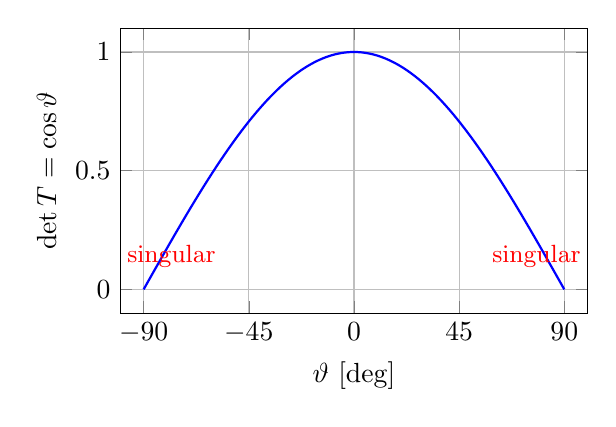
\begin{tikzpicture}
\begin{axis}[width=0.62\textwidth,height=5.2cm,xlabel={$\vartheta$ [deg]},ylabel={$\det T=\cos\vartheta$},
 xmin=-100,xmax=100,ymin=-0.1,ymax=1.1,xtick={-90,-45,0,45,90},grid=major,domain=-90:90,samples=100]
\addplot[thick,blue]{cos(x)};
\node[red,font=\small,anchor=south west] at (axis cs:55,0.05) {singular};
\node[red,font=\small,anchor=south east] at (axis cs:-55,0.05) {singular};
\end{axis}
\end{tikzpicture}
\caption{The determinant of $T(\Theta)$ vanishes when the pitch reaches $\pm 90^\circ$. (Original figure, not on the slides.)}
\end{figure}

\begin{intuition}
At $\vartheta=\pi/2$ we have $s_\vartheta=1$, $c_\vartheta=0$ and the relation becomes
$p=\dot\varphi-\dot\psi$, $(q,r)=\dot\vartheta\,(c_\varphi,-s_\varphi)$.
Two things go wrong. First, only the \emph{difference} $\dot\varphi-\dot\psi$ is visible: roll and yaw rotate about the same physical axis (the two gimbals are aligned, hence ``gimbal lock''), so we cannot tell them apart. Second, $(q,r)$ is always along one fixed direction: no choice of angle rates produces an arbitrary $(q,r)$. So the derivatives of the Euler angles \emph{cannot represent every angular velocity}. Close to the lock, to produce a normal $\Omega$ the angle rates must become huge: this is what we saw in DFL, where the yaw row of $J$ contains $1/\cos\vartheta$.
\end{intuition}

\begin{remark}
This is a property of the \emph{description}, not of the body. In fact \emph{every} 3-parameter representation of $SO(3)$ has singular points (reference [5], Stuelpnagel).
\end{remark}

\subsection{Axis--angle and unit quaternion (4 parameters) $\in S^3$ \sli{slide 4}}

\begin{definition}[Axis--angle, Rodrigues formula]
Rotating a frame by an angle $\theta$ (counter-clockwise, seen from the tip of $r$) about the unit vector $r$ ($\|r\|=1$) gives
\[
R(\theta,r)=rr^T+(I-rr^T)\cos\theta+S(r)\sin\theta ,
\]
where $S(r)=\hatm{r}$ is the skew-symmetric matrix of $r$ (see Section~\ref{sec:hat}).
\end{definition}

\begin{figure}[h]
\centering
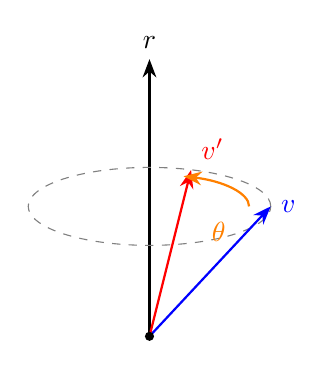
\begin{tikzpicture}[>=Stealth,scale=1.1]
\draw[->,thick] (0,0)--(0,3.2) node[above]{$r$};
\draw[dashed,gray] (0,1.5) ellipse (1.4 and 0.45);
\draw[->,thick,blue] (0,0)--(1.4,1.5) node[right]{$v$};
\draw[->,thick,red] (0,0)--(0.48,1.92) node[above right]{$v'$};
\draw[->,orange,thick] (1.15,1.5) arc[start angle=0,end angle=70,x radius=1.15,y radius=0.37];
\node[orange] at (0.8,1.2) {$\theta$};
\fill (0,0) circle (1.5pt);
\end{tikzpicture}
\caption{Rotating the vector $v$ by $\theta$ about the axis $r$ gives $v'=R(\theta,r)v$. (Redrawn from slide~4.)}
\end{figure}

Two facts about this representation:
\begin{itemize}
  \item the map $(\theta,r)\mapsto R$ is \textbf{not injective}: $R(\theta,r)=R(-\theta,-r)$;
  \item the inverse problem is
  \[
  \cos\theta=\frac{\tr R-1}{2},\qquad S(r)=\frac{R-R^T}{2\sin\theta},
  \]
  which is \textbf{singular for $\sin\theta=0$}.
\end{itemize}

\begin{definition}[Unit quaternion]
$\mathcal Q=\{\eta,\epsilon\}=\{\cos\tfrac\theta2,\ \sin\tfrac\theta2\,r\}$, with $\eta^2+\|\epsilon\|^2=1$ (a scalar $\eta$ and a 3-vector $\epsilon$). The associated rotation matrix is
\[
R(\eta,\epsilon)=(\eta^2-\epsilon^T\epsilon)I+2\epsilon\epsilon^T+2\eta\,S(\epsilon).
\]
\end{definition}
This is Rodrigues' formula again: $\eta^2-\|\epsilon\|^2=\cos\theta$, $2\epsilon\epsilon^T=(1-\cos\theta)rr^T$, $2\eta\epsilon=\sin\theta\,r$.

\begin{proposition}[Double covering]
The map from quaternions to rotations has no singularity in the inverse direction, but each physical attitude $R\in SO(3)$ is represented by a \textbf{pair of antipodal quaternions} $\pm\mathcal Q$. One says that $S^3$ is a \emph{double covering} of $SO(3)$.
\end{proposition}

\begin{intuition}
Because of the half angles, rotating by $\theta+2\pi$ gives $\cos(\tfrac\theta2+\pi)=-\cos\tfrac\theta2$: the quaternion changes sign, the rotation does not.
\emph{Numbers:} a $90^\circ$ rotation about $e_3$ has $\mathcal Q=(\cos45^\circ,\sin45^\circ e_3)=(0.707,\,0,0,0.707)$. The ``same'' rotation described as $450^\circ$ gives $(\cos225^\circ,\sin225^\circ e_3)=(-0.707,\,0,0,-0.707)=-\mathcal Q$. Same attitude, two different points of $S^3$.
\end{intuition}

\begin{figure}[h]
\centering
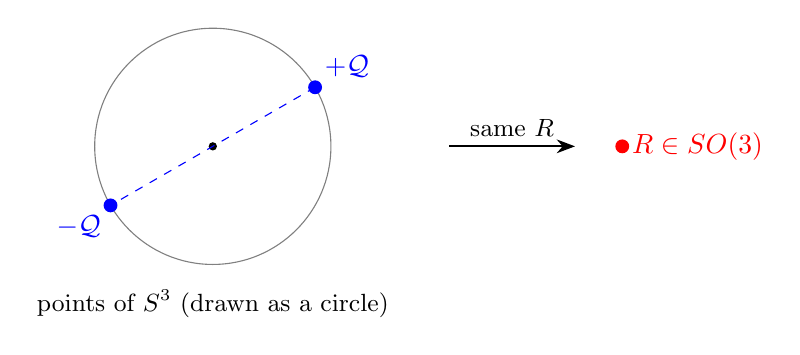
\begin{tikzpicture}[>=Stealth]
\draw[gray] (0,0) circle (1.5);
\fill (0,0) circle (1.5pt);
\fill[blue] (30:1.5) circle (2.5pt) node[above right]{$+\mathcal Q$};
\fill[blue] (210:1.5) circle (2.5pt) node[below left]{$-\mathcal Q$};
\draw[dashed,blue] (30:1.5)--(210:1.5);
\draw[->,thick] (3,0)--(4.6,0) node[midway,above]{\small same $R$};
\fill[red] (5.2,0) circle (2.5pt) node[right]{$R\in SO(3)$};
\node at (0,-2) {\small points of $S^3$ (drawn as a circle)};
\end{tikzpicture}
\caption{Two antipodal unit quaternions are the same attitude (analogy: $S^3$ drawn as a circle). Original figure.}
\end{figure}

\subsection{Rotation matrix (9 parameters) \sli{slide 5}}

\begin{definition}[$SO(3)$]
\[
SO(3)=\{R\in\R^{3\times3}:\ R^TR=I,\ \det R=+1\}.
\]
It uses 9 numbers with 6 independent constraints, so it is a \textbf{3-dimensional manifold}. For a body frame $RF_B$ seen from an inertial frame $RF_A$, the columns of ${}^A\!R_B=[\,{}^Ax_B\ {}^Ay_B\ {}^Az_B\,]$ are the body axes expressed in $RF_A$ (the \emph{direction cosines}).
\end{definition}

For the quadrotor $R=[\,b_1\ b_2\ b_3\,]$: the body axes expressed in the inertial frame. This is \textbf{one-to-one} with the physical attitudes.

\paragraph{The price.} $SO(3)$ is not a vector space: $R_1+R_2\notin SO(3)$ in general, and $R-R_d$ is not a sensible attitude error. Errors, derivatives and Lyapunov functions must respect the geometry.

\begin{intuition}
Example: $R_1=I$ and $R_2=R_z(\pi)=\diag(-1,-1,1)$ are both rotations, but $R_1+R_2=\diag(0,0,2)$ is not (it is not even invertible). Adding rotations is as meaningless as adding two points on a sphere and expecting to land on the sphere. What we do instead is \emph{multiply}: the relative rotation $R_d^TR$ plays the role of the difference $R-R_d$ (it is the identity exactly when $R=R_d$).
\end{intuition}

\subsection{Attitude representations: summary \sli{slide 6}}

\begin{center}
\small
\begin{tabular}{l l l l}
\toprule
representation & parameters & singularity-free? & unique? \\
\midrule
Euler angles (RPY) & 3 & NO ($\vartheta=\pm\pi/2$) & NO: $(\varphi,\vartheta,\psi)\sim(\varphi+\pi,\pi-\vartheta,\psi+\pi)$ \\
axis--angle & 4, $\|r\|=1$ & NO ($\sin\theta=0$) & NO: $(\theta,r)\sim(-\theta,-r)$ \\
unit quaternion & 4, $\|\mathcal Q\|=1$ & YES & NO: $\pm\mathcal Q$ \\
rotation matrix & 9, 6 constraints & YES & YES \\
\bottomrule
\end{tabular}
\end{center}

\begin{itemize}
  \item Non-uniqueness and singularities must be handled by the controller: errors and stability properties have to be reinterpreted on the set of physical attitudes $SO(3)$.
  \item Otherwise the closed loop can show the \emph{unwinding phenomenon} (next section).
\end{itemize}

% =====================================================================
\section{Why it matters for control \sli{slides 7--9}}

\subsection{Unwinding \sli{slide 7}}

Suppose we use quaternion feedback.
\begin{itemize}
  \item $+\mathcal Q$ and $-\mathcal Q$ are the same attitude but two different points of $S^3$.
  \item A continuous law that stabilizes $\mathcal Q=(1,0)$ treats $\mathcal Q=(-1,0)$ as a \emph{different} equilibrium.
  \item From initial conditions close to $-\mathcal Q$ the body may perform an unnecessary rotation of almost $2\pi$ before stopping: \textbf{unwinding}.
  \item Consequences: wasted control effort, large excursions after small perturbations (like a pendulum leaving its upright equilibrium).
  \item Fixing the sign (e.g.\ $\eta\ge0$) removes unwinding but makes the law \emph{discontinuous} at $\eta=0$: chattering with measurement noise [Mayhew et al.\ 2011].
  \item Further reading: [Bhat \& Bernstein 2000].
\end{itemize}

\begin{figure}[h]
\centering
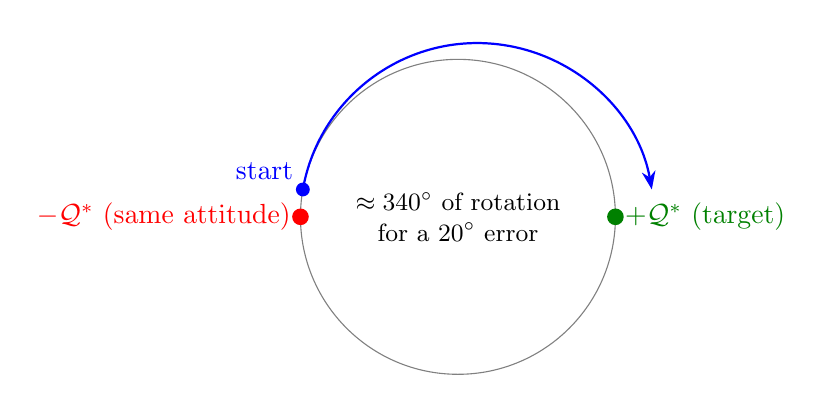
\begin{tikzpicture}[>=Stealth]
\draw[gray] (0,0) circle (2);
\fill[green!50!black] (0:2) circle (3pt) node[right]{$+\mathcal Q^\ast$ (target)};
\fill[red] (180:2) circle (3pt) node[left]{$-\mathcal Q^\ast$ (same attitude)};
\fill[blue] (170:2) circle (2.5pt) node[above left]{start};
\draw[->,thick,blue] (170:2) arc[start angle=170,end angle=10,radius=2.25];
\node[font=\small,align=center] at (0,0) {$\approx 340^\circ$ of rotation\\for a $20^\circ$ error};
\end{tikzpicture}
\caption{Unwinding, drawn on a circle that stands for $S^3$. A quaternion angle of $170^\circ$ means a rotation of $340^\circ$, i.e.\ only $20^\circ$ away from the target attitude, yet the controller goes the long way round. Original figure.}
\end{figure}

\begin{intuition}
Imagine the body is just $20^\circ$ away from where you want it. If the controller sees the ``wrong'' sign of the quaternion, it believes it is $340^\circ$ away and turns almost a full revolution the long way. A pendulum is a good picture: if you ask it to reach the hanging position and it starts just beyond the upright one, you want it to fall the short way, not to go around.
\end{intuition}

\subsection{Topology \sli{slide 8}}

\begin{theorem}[Topological obstruction, Bhat--Bernstein 2000]
The state space $SO(3)\times\R^3$ of the rotational dynamics is not homeomorphic to $\R^6$. Therefore \textbf{no continuous feedback} can make an equilibrium globally asymptotically stable. The best achievable with continuous feedback is \textbf{almost global} stability: convergence from all initial conditions except a set of measure zero.
\end{theorem}

Conclusion of the slide: design directly on $SO(3)$.
\begin{itemize}
  \item no representation singularities;
  \item no double covering, hence no unwinding;
  \item almost-global results: the best possible with continuous feedback;
  \item for the quadrotor this is the geometric controller of [1], whose configuration space is $SE(3)$.
\end{itemize}

\subsection{Why some attitudes must be left out \sli{slide 9}}

Attitudes live on a closed set ($360^\circ=0^\circ$). The slide explains the obstruction with a one-dimensional example.

\begin{proposition}[1-D version of the obstruction]
Let $\theta\in S^1=\R/2\pi\mathbb{Z}$ be an angle and $u(\theta)$ a continuous feedback (a torque) that makes $\theta=0$ locally stable. Then $u$ has at least one more zero, at some $\theta^\ast\ne 0$, i.e.\ a second equilibrium.
\end{proposition}
\begin{proof}
Stability of $0$ means $u<0$ just to the right of $0$ and $u>0$ just to the left. Going around the circle from $0^+$ (where $u<0$) to $2\pi^-\equiv0^-$ (where $u>0$), by the intermediate value theorem $u$ vanishes somewhere in between.
\end{proof}

\begin{figure}[h]
\centering
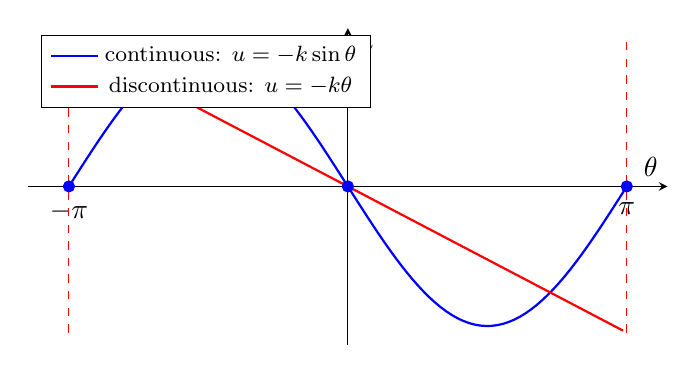
\begin{tikzpicture}
\begin{axis}[width=0.8\textwidth,height=5.6cm,xlabel={$\theta$},ylabel={$u$},xmin=-3.6,xmax=3.6,ymin=-3.4,ymax=3.4,
  xtick={-3.14159,0,3.14159},xticklabels={$-\pi$,$0$,$\pi$},ytick=\empty,axis lines=middle,
  legend style={at={(0.02,0.98)},anchor=north west,font=\footnotesize},samples=100]
\addplot[thick,blue,domain=-3.14159:3.14159]{-3*sin(deg(x))};
\addlegendentry{continuous: $u=-k\sin\theta$}
\addplot[thick,red,domain=-3.1:3.1]{-x};
\addlegendentry{discontinuous: $u=-k\theta$}
\draw[red,dashed] (axis cs:3.14159,-3.14159)--(axis cs:3.14159,3.14159);
\draw[red,dashed] (axis cs:-3.14159,-3.14159)--(axis cs:-3.14159,3.14159);
\addplot[only marks,mark=*,blue] coordinates {(0,0) (3.14159,0) (-3.14159,0)};
\end{axis}
\end{tikzpicture}
\caption{Feedback on a circle. The smooth law is forced to vanish again at $\theta=\pm\pi\ (\equiv)$; the law $-k\theta$ avoids this only by jumping at $\pm\pi$ (chattering). Original figure, same idea as slide~9(b).}
\end{figure}

In $SO(3)$ the same happens: the torque $-k_R\eR$ of the geometric controller, with $\|\eR\|=\sin\theta$, vanishes at the target \emph{and} at the $180^\circ$ errors.

\begin{intuition}
Picture a ball on a smooth hill-and-valley landscape drawn on a circle. If there is a valley at the target, going around the circle there must be a hilltop somewhere else. At the hilltop the ball can sit still: that is the $180^\circ$ error, a rotation exactly upside down relative to the target, where the controller has no preferred direction to turn (both ways are equally long). Starting anywhere except exactly on the hilltop the ball rolls to the valley, which is why the result is ``almost global''.
\end{intuition}

% =====================================================================
\section{A globally defined model on $SE(3)$ \sli{slides 10--11}}
\label{sec:model}

\subsection{The model \sli{slide 10}}

\begin{definition}[Quadrotor on $SE(3)$]
\begin{align*}
\dot x&=v,\\
m\dot v&=mg\,e_3-f\,Re_3,\\
\dot R&=R\,\hatm{\Omega},\\
J\dot\Omega+\Omega\times J\Omega&=M,
\end{align*}
with $f=\sum_{i=1}^4f_i$ and $M=(\tau_\varphi,\tau_\vartheta,\tau_\psi)^T$.
\end{definition}

\begin{itemize}
  \item Same model as in the previous lectures: NED frame ($e_3$ points down), thrust along $-b_3=-Re_3$; $f\equiv T$, $J\equiv\diag(I_x,I_y,I_z)$, $M\equiv\Gamma$ are torques about the \emph{body} axes.
  \item Configuration $(x,R)\in SE(3)=\R^3\times SO(3)$, state $(x,v,R,\Omega)$: \textbf{12-dimensional} (3+3+3+3).
  \item No local coordinates: the model is valid for \emph{every} attitude.
  \item $(f,M)$ and the rotor thrusts $f_i$ are related by an invertible linear map (Lecture~1), so we may treat $(f,M)$ as the inputs.
\end{itemize}

\begin{figure}[h]
\centering
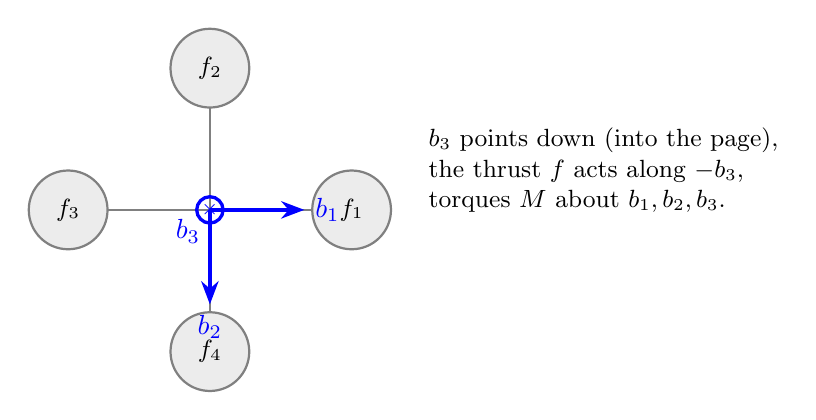
\begin{tikzpicture}[>=Stealth,scale=1.0]
\foreach \a/\n in {0/1,90/2,180/3,270/4}{
  \draw[thick,gray] (0,0)--(\a:1.8);
  \draw[thick,gray,fill=gray!15] (\a:1.8) circle (0.5);
  \node at (\a:1.8) {\small $f_{\n}$};
}
\draw[->,very thick,blue] (0,0)--(1.2,0) node[right]{$b_1$};
\draw[->,very thick,blue] (0,0)--(0,-1.2) node[below]{$b_2$};
\node[circle,draw,blue,inner sep=0.5pt,very thick] at (0,0) {\scriptsize $\times$};
\node[blue,below left] at (0,0) {$b_3$};
\node[font=\small,align=left] at (5,0.5) {$b_3$ points down (into the page),\\ the thrust $f$ acts along $-b_3$,\\ torques $M$ about $b_1,b_2,b_3$.};
\end{tikzpicture}
\caption{Schematic top view of the quadrotor and its body axes (simplified; original figure, the slide shows a 3D rendering with $R$, $x$, $\vec e_i$, $\vec b_i$).}
\end{figure}

\subsection{Kinematics on $SO(3)$: the hat map \sli{slide 11}}
\label{sec:hat}

\begin{definition}[Hat and vee maps]
The \emph{hat map} $\hatm{\cdot}:\R^3\to so(3)$ (skew-symmetric matrices) is
\[
\hatm{x}=S(x)=\begin{pmatrix}0&-x_3&x_2\\x_3&0&-x_1\\-x_2&x_1&0\end{pmatrix},\qquad \hatm{x}y=x\times y,\qquad(\hatm{x})\VEE=x.
\]
Its inverse is the \emph{vee map} $(\cdot)\VEE$.
\end{definition}

\begin{proposition}[Kinematic equation]
Let $R(t)\in SO(3)$. Then $R^T\dot R=:\hatm\Omega$ is skew-symmetric, so
\[
\dot R=R\hatm\Omega=\hatm\omega R,\qquad \omega=R\Omega .
\]
$\Omega$ is the angular velocity expressed in the \textbf{body} frame, $\omega$ in the \textbf{inertial} frame.
\end{proposition}
\begin{proof}
Differentiate $R^TR=I$: $R^T\dot R+\dot R^TR=0$, i.e.\ $R^T\dot R=-(R^T\dot R)^T$. The equality $R\hatm\Omega=\hatm\omega R$ follows from $R\hatm\Omega R^T=\widehat{R\Omega}$.
\end{proof}

\begin{intuition}
The hat map turns a cross product into a matrix multiplication, so rotation algebra becomes matrix algebra. Example: $x=(1,2,3)^T$ gives $\hatm x=\begin{psmallmatrix}0&-3&2\\3&0&-1\\-2&1&0\end{psmallmatrix}$. The relation $\dot R=R\hatm\Omega$ says: the columns $b_i$ of $R$ move like rigid arrows, $\dot b_i=\omega\times b_i$. Writing the same rotation in the body frame ($\Omega$) or in the inertial frame ($\omega=R\Omega$) is just a change of basis.
\end{intuition}

% =====================================================================
\section{Controller structure \sli{slides 12--14}}

\subsection{Controller structure \sli{slide 12}}

\begin{figure}[h]
\centering
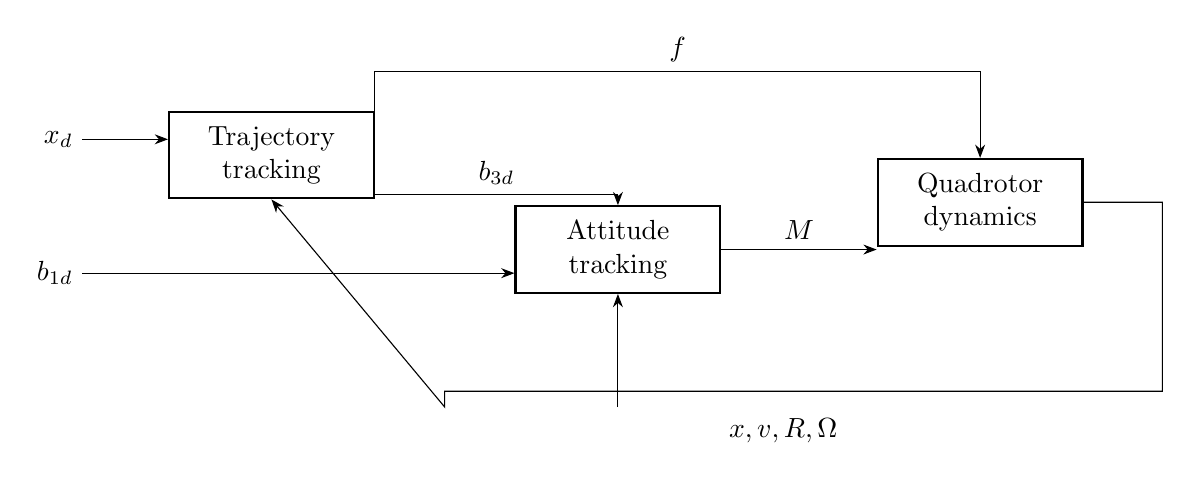
\begin{tikzpicture}[>=Stealth,block/.style={draw,thick,rectangle,minimum width=2.6cm,minimum height=1.1cm,align=center}]
\node[block] (traj) at (0,0) {Trajectory\\tracking};
\node[block] (att) at (4.4,-1.2) {Attitude\\tracking};
\node[block] (quad) at (9,-0.6) {Quadrotor\\dynamics};
\draw[->] (-2.4,0.2)--(traj.west |- 0,0.2) node[pos=0,left]{$x_d$};
\draw[->] (-2.4,-1.5)--(att.west |- 0,-1.5) node[pos=0,left]{$b_{1d}$};
\draw[->] (traj.east |- 0,-0.5)-|(att.north) node[pos=0.25,above]{$b_{3d}$};
\draw[->] (traj.north east)--++(0,0.5)-|(quad.north) node[pos=0.25,above]{$f$};
\draw[->] (att.east)--(quad.west |- att.east) node[midway,above]{$M$};
\draw[->] (quad.east)--++(1,0)--++(0,-2.4)-|(2.2,-3.2)--(traj.south) ;
\draw[->] (4.4,-3.2)--(att.south);
\node at (6.5,-3.5) {$x,v,R,\Omega$};
\end{tikzpicture}
\caption{Block structure: the position loop produces the thrust magnitude $f$ and the desired thrust direction $b_{3d}$; the attitude loop produces the moment $M$. (Redrawn from slide~12; arrows simplified.)}
\end{figure}

\begin{itemize}
  \item \textbf{Tracked outputs:} position $x_d(t)\in\R^3$ and heading direction $b_{1d}(t)\in S^2$ (4 outputs, like $(x,y,z,\psi)$ in DFL).
  \item \textbf{Trajectory tracking:} gives the thrust magnitude $f$ and the desired thrust direction $b_{3d}$.
  \item \textbf{Attitude tracking:} gives the moment $M$ to track $R_d$, built from $b_{3d}$ and $b_{1d}$.
  \item The structure is hierarchical, but \textbf{no time-scale separation} is assumed: stability is proved for the \emph{complete} loop.
  \item Tracking errors: $\ex=x-x_d$, $\ev=v-v_d$, with $v_d=\dot x_d$.
\end{itemize}

\subsection{Thrust magnitude and direction \sli{slide 13}}

Define the \emph{ideal force} (PD + gravity compensation + feedforward, as in Lecture~2)
\[
A:=-k_x\ex-k_v\ev-mg\,e_3+m\ddot x_d .
\]
If the thrust force $-fRe_3$ were equal to $A$, then $m\dot v-m\ddot x_d=mge_3+A-m\ddot x_d$, that is
\[
m\dot e_v=-k_x\ex-k_v\ev ,
\]
a stable linear error equation. But we cannot produce any force we like: the thrust acts only along the body axis $-b_3=-Re_3$.

\begin{definition}[Thrust magnitude and desired direction]
\[
b_{3d}=-\frac{A}{\|A\|},\qquad f=-A\cdot Re_3=\|A\|\,(b_{3d}\cdot b_3)=\|A\|\cos\alpha ,
\]
where $\alpha$ is the angle between the actual thrust axis $b_3$ and the desired one $b_{3d}$.
\end{definition}

So $f$ is the \emph{projection} of the desired force on the current thrust axis. It is reduced when $b_3\ne b_{3d}$, and $f>0\iff\alpha<90^\circ$.

\paragraph{Assumptions.} $\|A\|\ne0$ (no free-fall command, the analogue of $T\neq0$ in DFL) and a bounded reference, $\|-mge_3+m\ddot x_d\|\le B$.

\begin{figure}[h]
\centering
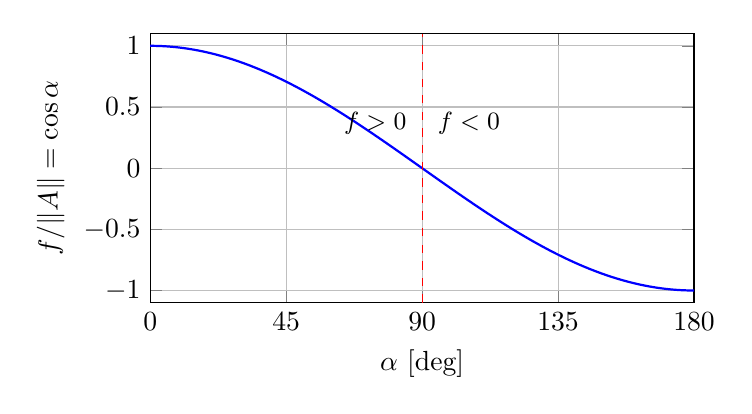
\begin{tikzpicture}
\begin{axis}[width=0.7\textwidth,height=5cm,xlabel={$\alpha$ [deg]},ylabel={$f/\|A\|=\cos\alpha$},xmin=0,xmax=180,ymin=-1.1,ymax=1.1,
 xtick={0,45,90,135,180},grid=major,domain=0:180,samples=100]
\addplot[thick,blue]{cos(x)};
\draw[red,dashed] (axis cs:90,-1.1)--(axis cs:90,1.1);
\node[font=\small,anchor=south west] at (axis cs:92,0.2) {$f<0$};
\node[font=\small,anchor=south east] at (axis cs:88,0.2) {$f>0$};
\end{axis}
\end{tikzpicture}
\caption{The thrust shrinks as the body axis moves away from the desired one and changes sign beyond $90^\circ$. Original figure.}
\end{figure}

\begin{intuition}
You want to push the drone up with force $\|A\|$ but the propellers point $60^\circ$ away from that direction. Only the component along the propeller axis is useful, so you command $f=\|A\|\cos60^\circ=\|A\|/2$: less thrust while the vehicle is still tilting into place, instead of pushing hard in the wrong direction. At $90^\circ$ the thrust is zero, beyond that the formula asks for negative thrust (a reversible propeller), which we will meet again in the simulation.
\end{intuition}

\subsection{Reference attitude \sli{slide 14}}

Given $b_{1d}$ and the computed $b_{3d}$, define
\[
b_{2d}=\frac{b_{3d}\times b_{1d}}{\|b_{3d}\times b_{1d}\|},\qquad
\boxed{R_d=[\,b_{2d}\times b_{3d},\ b_{2d},\ b_{3d}\,]\in SO(3)}
\]

\begin{lemma}
$R_d$ is well defined iff $b_{1d}\nparallel b_{3d}$, and then $R_d\in SO(3)$. Its first axis is the normalized \emph{projection} of $b_{1d}$ on the plane normal to $b_{3d}$.
\end{lemma}
\begin{proof}
$b_{2d}$ needs $b_{3d}\times b_{1d}\ne0$. By construction $b_{2d}\perp b_{3d}$ and both are unit vectors, so $b_1'=b_{2d}\times b_{3d}$ completes a right-handed orthonormal triad ($b_1'\times b_{2d}=b_{3d}$). Using $(a\times b)\times c=b(a\cdot c)-a(b\cdot c)$,
\[
b_{2d}\times b_{3d}=\frac{(b_{3d}\times b_{1d})\times b_{3d}}{\|b_{3d}\times b_{1d}\|}=\frac{b_{1d}-(b_{3d}\cdot b_{1d})\,b_{3d}}{\|b_{3d}\times b_{1d}\|},
\]
which is $b_{1d}$ minus its component along $b_{3d}$, normalized.
\end{proof}

\begin{figure}[h]
\centering
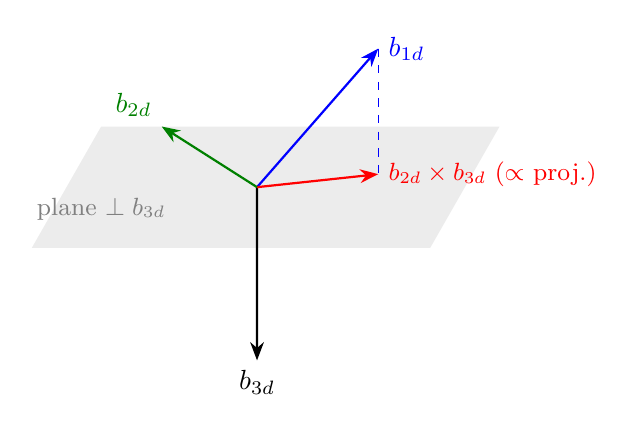
\begin{tikzpicture}[>=Stealth,scale=1.1]
\fill[gray!15] (-2,-0.4)--(2.6,-0.4)--(3.4,1)--(-1.2,1)--cycle;
\node[gray] at (-1.2,0.05) {\small plane $\perp b_{3d}$};
\coordinate (O) at (0.6,0.3);
\draw[->,thick] (O)--(0.6,-1.7) node[below]{$b_{3d}$};
\draw[->,thick,blue] (O)--(2.0,1.9) node[right]{$b_{1d}$};
\draw[dashed,blue] (2.0,1.9)--(2.0,0.45);
\draw[->,thick,red] (O)--(2.0,0.45) node[right]{\small $b_{2d}\times b_{3d}$ ($\propto$ proj.)};
\draw[->,thick,green!50!black] (O)--(-0.5,1.0) node[above left]{$b_{2d}$};
\end{tikzpicture}
\caption{Construction of $R_d$. The first axis is the projection of $b_{1d}$ on the plane normal to $b_{3d}$ (redrawn and simplified from slide~14).}
\end{figure}

\begin{itemize}
  \item $b_{1d}$ need not be orthogonal to $b_{3d}$: only its projection is tracked.
  \item The desired angular velocity is defined by $\hatm\Omega_d=R_d^T\dot R_d$.
\end{itemize}

\begin{intuition}
Two directions fix an orientation: ``where the propellers must point'' ($b_{3d}$, dictated by the force we need) and ``where the nose should roughly look'' ($b_{1d}$, a free choice). Because the nose direction is not perpendicular to the thrust axis in general, we take the closest legal choice: the shadow of $b_{1d}$ on the plane perpendicular to $b_{3d}$. This is possible unless $b_{1d}$ is exactly parallel to $b_{3d}$ (looking straight along the thrust), where the shadow is a point and the heading is undefined.
\end{intuition}

% =====================================================================
\section{Attitude errors and the attitude controller \sli{slides 15--20}}

\subsection{Attitude error function \sli{slide 15}}

\begin{definition}[Attitude error function]
\[
\Psi(R,R_d)=\tfrac12\tr\!\big[I-R_d^TR\big],\qquad\text{defined on }SO(3)\times SO(3).
\]
\end{definition}

The matrix $R_d^TR$ is a rotation by an angle $\theta\in[0,\pi]$ about some axis $r$, so $\tr(R_d^TR)=1+2\cos\theta$ and
\[
\Psi=1-\cos\theta\in[0,2],\qquad \Psi=\tfrac14\|R-R_d\|_F^2 .
\]
\begin{itemize}
  \item $\Psi=0\iff R=R_d$; $\ \Psi<1\iff\theta<90^\circ$; $\ \Psi=2\iff\theta=180^\circ$.
  \item $\Psi$ is positive definite about $R=R_d$, and it is bounded by quadratic functions of the attitude error (Lemma below) on the sublevel sets $\{\Psi\le\psi_2<2\}$, i.e.\ for rotation errors smaller than $180^\circ$.
  \item The sublevel set $L_2=\{R_d,R\in SO(3)\mid\Psi(R,R_d)<2\}$ excludes only the $180^\circ$ errors: it \emph{almost covers} $SO(3)$ (the complement has zero measure).
\end{itemize}

\begin{figure}[h]
\centering
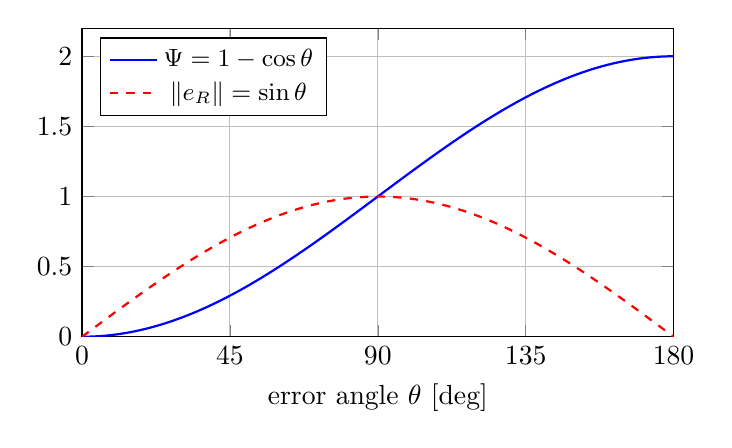
\begin{tikzpicture}
\begin{axis}[width=0.75\textwidth,height=5.5cm,xlabel={error angle $\theta$ [deg]},xmin=0,xmax=180,ymin=0,ymax=2.2,
 xtick={0,45,90,135,180},grid=major,domain=0:180,samples=100,legend style={at={(0.03,0.97)},anchor=north west,font=\small}]
\addplot[thick,blue]{1-cos(x)};\addlegendentry{$\Psi=1-\cos\theta$}
\addplot[thick,red,dashed]{sin(x)};\addlegendentry{$\|e_R\|=\sin\theta$}
\end{axis}
\end{tikzpicture}
\caption{The error function $\Psi$ grows monotonically up to $180^\circ$, while the gradient norm $\|e_R\|=\sin\theta$ rises and then falls back to zero (Section~\ref{sec:eR}). Original figure.}
\end{figure}

\begin{intuition}
$\Psi$ is a ``distance'' between two attitudes that works on the manifold: $0$ when they coincide, $1$ at a right angle, $2$ when the body is upside down relative to the target. In numbers: $\theta=60^\circ\Rightarrow\Psi=0.5$; $\theta=90^\circ\Rightarrow\Psi=1$; $\theta=178^\circ\Rightarrow\Psi\approx1.9994$ (the value used in the simulation of slide~28).
\end{intuition}

\subsection{Attitude tracking error \sli{slide 16}}
\label{sec:eR}

Perturb $R$ as $R\exp(\hatm\eta)$ with $\eta\in\R^3$ (body frame): $\delta R=R\hatm\eta$ and
\[
\delta\Psi=-\tfrac12\tr\big(R_d^TR\,\hatm\eta\big)=\tfrac12\,\eta^T\big(R_d^TR-R^TR_d\big)\VEE=\eR\cdot\eta .
\]

\begin{definition}[Attitude error vector]
\[
\eR=\tfrac12\big(R_d^TR-R^TR_d\big)\VEE\in\R^3 ,
\]
the gradient of $\Psi$.
\end{definition}

Using $R_d^TR=\exp(\theta\hatm r)=I+\sin\theta\,\hatm r+(1-\cos\theta)\hatm r^2$ we get $R_d^TR-R^TR_d=2\sin\theta\,\hatm r$, hence
\[
\eR=\sin\theta\;r ,
\]
and for small errors $\eR\simeq\theta r$, the rotation vector.

\begin{lemma}[Bounds]
$\|\eR\|^2=\sin^2\theta=\Psi(2-\Psi)$. Hence on $\{\Psi\le\psi_2<2\}$
\[
\tfrac12\|\eR\|^2\le\Psi\le\frac1{2-\psi_2}\|\eR\|^2 .
\]
\end{lemma}
\begin{proof}
$\sin^2\theta=(1-\cos\theta)(1+\cos\theta)=\Psi(2-\Psi)$. Since $2-\Psi\le2$ we get $\|\eR\|^2\le2\Psi$; since $2-\Psi\ge2-\psi_2$ we get $\|\eR\|^2\ge(2-\psi_2)\Psi$.
\end{proof}

\begin{remark}
$\eR=0$ also for $\theta=\pi$. The critical points of $\Psi$ are $R=R_d$ and the $180^\circ$ errors: these are \emph{undesired equilibria of any gradient-like attitude controller}.
\end{remark}

\begin{intuition}
$\eR$ tells the controller ``about which axis, and how strongly, to turn'': the axis is the rotation axis $r$ of the error, the strength is $\sin\theta$. For a small error it is just $\theta$ (like the ordinary error $x-x_d$). Note the catch: $\sin\theta$ is \emph{small} near $\theta=180^\circ$, e.g.\ $\sin178^\circ=0.035$. A drone that is almost upside down feels almost no push to turn, which explains why it leaves that configuration slowly (slide~28).
\end{intuition}

\subsection{Angular velocity tracking error \sli{slide 17}}

\begin{definition}
\[
\eO=\Omega-R^TR_d\,\Od .
\]
\end{definition}

$\Omega$ is expressed in the body frame of $R$, while $\Od$ is expressed in the body frame of $R_d$. The vector $R_d\Od$ is the desired angular velocity in the inertial frame, and $R^TR_d\Od$ the same vector in the \emph{current} body frame; only then can the two be subtracted.

\begin{proposition}
$\eO$ is the angular velocity of the relative rotation $R_d^TR$:
\[
\frac{d}{dt}\big(R_d^TR\big)=R_d^TR\,\hatm{\eO}.
\]
\end{proposition}
\begin{proof}
With $\dot R_d=R_d\hatm\Od$ and $\dot R=R\hatm\Omega$,
\[
\frac d{dt}(R_d^TR)=\dot R_d^TR+R_d^T\dot R=-\hatm\Od R_d^TR+R_d^TR\hatm\Omega
=R_d^TR\big(\hatm\Omega-R^TR_d\hatm\Od R_d^TR\big)=R_d^TR\,\big(\Omega-R^TR_d\Od\big)^\wedge ,
\]
using $Q\hatm xQ^T=\widehat{Qx}$ with $Q=R^TR_d$.
\end{proof}

The signals $\Od$ and $\dot\Omega_d$ come from $R_d(t)$: $\hatm\Od=R_d^T\dot R_d$.

\begin{intuition}
It is the same idea as the velocity error $v-v_d$, but we have to compare two angular velocities written in two different frames (the real body frame and the desired one). Rewriting the desired one in the current body frame is the ``translation'' $R^TR_d$ that makes the subtraction meaningful.
\end{intuition}

\subsection{Error kinematics \sli{slide 18}}

\paragraph{Attitude error function.} 
\[
\dot\Psi=-\tfrac12\tr\!\Big(\tfrac d{dt}(R_d^TR)\Big)=-\tfrac12\tr\big(R_d^TR\,\hatm{\eO}\big)=\tfrac12\,\eO^T\big(R_d^TR-R^TR_d\big)\VEE,
\qquad\boxed{\dot\Psi=\eR\cdot\eO}.
\]

\paragraph{Attitude error vector.}
\[
\dot\eR=\tfrac12\big(R_d^TR\,\hatm{\eO}+\hatm{\eO}\,R^TR_d\big)\VEE=\tfrac12\big(\tr(R^TR_d)I-R^TR_d\big)\eO=:C(R_d^TR)\,\eO,\qquad\|C\|\le1,
\]
(by the identity $\hatm xA+A^T\hatm x=\big((\tr A\,I-A)x\big)^\wedge$ with $A=R^TR_d$).

\paragraph{Angular velocity error.} Since $\hatm\Od\Od=0$,
\[
\frac d{dt}\big(R^TR_d\Od\big)=-\hatm\Omega R^TR_d\Od+R^TR_d\hatm\Od\Od+R^TR_d\dot\Omega_d,
\qquad
\dot\eO=\dot\Omega+\hatm\Omega R^TR_d\Od-R^TR_d\dot\Omega_d .
\]

\begin{intuition}
The first formula says: the error function changes only if the body is turning relative to the target ($\eO$) \emph{and} the error has a gradient ($\eR$). The matrix $C$ is a ``gain'' of norm at most 1: a rotation error that is turning at rate $\eO$ changes its vector $\eR$ at a rate that is never larger than $\|\eO\|$ (it is the exact analogue of $\dot e=e_{\text{velocity}}$ in a double integrator, but $\le1$ because of the geometry).
\end{intuition}

\subsection{Attitude tracking controller \sli{slide 19}}

Multiply the last equation by $J$ and use $J\dot\Omega=M-\Omega\times J\Omega$:
\[
J\dot\eO=M-\Omega\times J\Omega+J\big(\hatm\Omega R^TR_d\Od-R^TR_d\dot\Omega_d\big).
\]

\begin{definition}[Tracking controller on $SO(3)$]
\[
M=-k_R\eR-k_\Omega\eO+\Omega\times J\Omega-J\big(\hatm\Omega R^TR_d\Od-R^TR_d\dot\Omega_d\big).
\]
\end{definition}

Closed-loop attitude error dynamics:
\[
J\dot\eO=-k_R\eR-k_\Omega\eO,\qquad\dot\eR=C(R_d^TR)\,\eO,\qquad \tfrac d{dt}(R_d^TR)=R_d^TR\,\hatm{\eO}.
\]
It is a \emph{computed torque}: cancellation of the gyroscopic term and feedforward of the desired angular acceleration, plus a PD action on $SO(3)$. The closed loop is \textbf{autonomous} in $(R_d^TR,\eO)$: it does not depend on the translational motion.

\begin{intuition}
Strip everything away and the law is $J\dot\eO=-k_R\eR-k_\Omega\eO$: a rotational spring ($k_R$ pulls the attitude toward $R_d$) and a damper ($k_\Omega$ kills the relative angular velocity), acting on a body of inertia $J$. All the other terms are there only to cancel what the real dynamics add (the $\Omega\times J\Omega$ coupling and the motion of the reference), so that this clean mass--spring--damper behaviour remains.
\end{intuition}

\subsection{Attitude dynamics: stability \sli{slide 20}}

Take $V=\tfrac12\eO^TJ\eO+k_R\Psi$ (kinetic energy of the error plus potential energy). Then
\[
\dot V=\eO^T(-k_R\eR-k_\Omega\eO)+k_R\,\eR\cdot\eO=-k_\Omega\|\eO\|^2\le0 .
\]
If $V(0)<2k_R$ then $k_R\Psi(t)\le V(t)\le V(0)<2k_R$, so $\Psi<2$ forever: the error never reaches $180^\circ$. This holds if
\[
\|\eO(0)\|^2<\frac{2k_R}{\lmax(J)}\big(2-\Psi(0)\big).
\]
For exponential convergence one adds a cross term: $V_2=\tfrac12\eO^TJ\eO+k_R\Psi+c_2\,\eR\cdot\eO$, and using $\|C\|\le1$,
\[
\dot V_2\le-(k_\Omega-c_2)\|\eO\|^2-\frac{c_2k_R}{\lmax(J)}\|\eR\|^2+\frac{c_2k_\Omega}{\lmin(J)}\|\eR\|\|\eO\|=-z_2^TW_2z_2,\quad z_2=(\|\eR\|,\|\eO\|)^T ,
\]
with $W_2>0$ for $c_2$ small enough; on $\{\Psi\le\psi_2<2\}$, $V_2$ lies between two quadratic forms of $z_2$.

\begin{proposition}[Attitude, Proposition 1 of [1]]
If $\Psi(R(0),R_d(0))<2$ and $\|\eO(0)\|^2<\frac{2k_R}{\lmax(J)}\big(2-\Psi(R(0),R_d(0))\big)$, then the zero equilibrium of the attitude tracking errors is \textbf{exponentially stable}: $\eR,\eO\to0$ exponentially (initial attitude error below $180^\circ$).
\end{proposition}

\begin{intuition}
$V$ is the total energy of the ``rotational spring--damper'': the damper only dissipates energy, so $V$ never increases. Since $\Psi=2$ would cost $2k_R$ of potential energy, if the initial energy is below $2k_R$ the system simply does not have enough energy to climb to the $180^\circ$ hilltop. The cross term $c_2\eR\cdot\eO$ is the usual trick to turn ``it stops moving'' ($\dot V\le0$ only in $\eO$) into ``it converges exponentially''. 
\end{intuition}

% =====================================================================
\section{Position error and the complete system \sli{slides 21--24}}

\subsection{Position error dynamics \sli{slide 21}}

We have $m\dot\ev=mge_3-fRe_3-m\ddot x_d$. Add and subtract the force along $b_{3d}$:
\[
-fRe_3=-\frac f{b_{3d}\cdot b_3}\,b_{3d}-X,\qquad X:=\frac f{b_{3d}\cdot b_3}\Big((b_{3d}\cdot b_3)\,b_3-b_{3d}\Big).
\]
Since $f=\|A\|(b_{3d}\cdot b_3)$ and $-\|A\|b_{3d}=A$,
\[
\boxed{m\dot\ev=-k_x\ex-k_v\ev-X}.
\]

\begin{lemma}[Bound on the coupling term]
$X=0$ when $b_3=b_{3d}$. Moreover $\|(b_{3d}\cdot b_3)b_3-b_{3d}\|=\sin\alpha$ and $\alpha\le\theta$, so for $\Psi<1$ ($\theta<90^\circ$)
\[
\|X\|\le\big(k_x\|\ex\|+k_v\|\ev\|+B\big)\|\eR\|,
\]
with $\|\eR\|\le\sqrt{\psi_1(2-\psi_1)}<1$ on $\{\Psi\le\psi_1<1\}$. For $\Psi<1$ also $\alpha<90^\circ$, hence $f>0$.
\end{lemma}

(The bound follows because $X=\|A\|\big((b_{3d}\cdot b_3)b_3-b_{3d}\big)$ and $\|A\|\le k_x\|\ex\|+k_v\|\ev\|+B$.)

\begin{intuition}
$X$ is the ``leakage'': the part of the desired force that is lost because the propellers are not yet pointing the right way. It is zero when the attitude is right, and proportional to the attitude error when it is not. So the position error behaves like a stable linear system $m\dot\ev=-k_x\ex-k_v\ev$ driven by a disturbance $X$ that dies with the attitude error: ``if there is no attitude error, the position error converges''. The dot product in $f$ also reduces the thrust when the axes separate and keeps it positive in the region where the analysis of the complete system holds.
\end{intuition}

\subsection{Complete dynamics: exponential stability \sli{slide 22}}

The structure is a \textbf{cascade}: the attitude error subsystem is autonomous and drives the position error subsystem through $X$.

\begin{figure}[h]
\centering
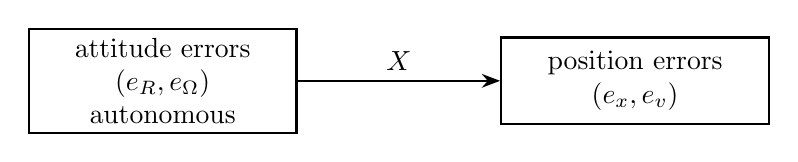
\begin{tikzpicture}[>=Stealth,block/.style={draw,thick,minimum width=3.4cm,minimum height=1.1cm,align=center}]
\node[block] (a) at (0,0) {attitude errors\\$(\eR,\eO)$ \\ autonomous};
\node[block] (p) at (6,0) {position errors\\$(\ex,\ev)$};
\draw[->,thick] (a)--(p) node[midway,above]{$X$};
\end{tikzpicture}
\caption{Cascade structure of the closed loop. Original figure.}
\end{figure}

Take $V_1=\tfrac12k_x\|\ex\|^2+\tfrac1{2m}\|\ev\|^2+c_1\,\ex\cdot\ev$ and $V=V_1+V_2$. Then
\[
\dot V\le-z_1^TW_1z_1+z_1^TW_{12}z_2-z_2^TW_2z_2,\qquad z_1=(\|\ex\|,\|\ev\|)^T,
\]
where $W_{12}$ collects the bound on $X$ and is bounded on the domain $\|\ex\|<e_{x,\max}$. The right side is negative definite iff
\[
4\lmin(W_1)\lmin(W_2)>\|W_{12}\|^2 .
\]
This means that the attitude gains $k_R,k_\Omega$ must be large enough with respect to the position loop: a provable version of the rule ``\emph{inner loop faster than outer loop}'' of Lecture~2.

\begin{proposition}[Complete system, Proposition 2 of [1]]
For any $k_x,k_v>0$ there exist $c_1,c_2,k_R,k_\Omega$ (explicit conditions in [1]) such that, if $\Psi(R(0),R_d(0))<\psi_1<1$, $\|\ex(0)\|<e_{x,\max}$ and $\|\eO(0)\|$ is small enough, the zero equilibrium of the tracking errors of the complete system is \textbf{exponentially stable} (initial attitude error below $90^\circ$).
\end{proposition}

\begin{intuition}
Think of two coupled quadratic ``bowls'': position and attitude. The attitude bowl pushes on the position one (through $X$) with strength proportional to its own size. If the attitude bowl is steep enough (large $k_R,k_\Omega$), it empties faster than it can disturb the position, and both converge. The inequality $4\lmin(W_1)\lmin(W_2)>\|W_{12}\|^2$ is just the condition for a $2\times2$ quadratic form $\begin{psmallmatrix}a&-b/2\\-b/2&c\end{psmallmatrix}$ to be positive definite ($4ac>b^2$).
\end{intuition}

\subsection{Almost global exponential attractiveness \sli{slide 23}}

\begin{itemize}
  \item From any $\Psi(0)<2$ (with the bound on $\eO(0)$ of Proposition 1) the attitude error decreases exponentially and enters $\{\Psi\le\psi_1\}$ at a finite time $t^\ast$.
  \item On $[0,t^\ast]$ the position errors remain bounded: $\|X\|$ grows at most linearly with $\|\ex\|,\|\ev\|$, so there is no finite escape time.
  \item After $t^\ast$ Proposition 2 applies.
\end{itemize}

\begin{proposition}[Proposition 3 of [1]]
If $\Psi(R(0),R_d(0))<2$ and $\|\eO(0)\|^2<\frac{2k_R}{\lmax(J)}\big(2-\Psi(R(0),R_d(0))\big)$, the zero equilibrium of the tracking errors of the complete system is \textbf{exponentially attractive}.
\end{proposition}

Since $L_2$ almost covers $SO(3)$, this is \emph{almost global exponential attractiveness}, the best possible with continuous feedback.

\begin{intuition}
Phase 1: the attitude loop first brings the error from, say, $170^\circ$ down below $90^\circ$ (the position may wander, but not explode). Phase 2: from there Proposition 2 takes over, with a guaranteed exponential rate. The word ``attractive'' (and not ``stable'') is used because during phase 1 the errors may grow before decreasing, so we cannot bound them by their initial value.
\end{intuition}

\subsection{Controller stability properties: summary \sli{slide 24}}

\begin{center}
\small
\begin{tabular}{l l l}
\toprule
initial attitude error & subsystem & property \\
\midrule
$\Psi<2$ ($\theta<180^\circ$) & attitude & exponential stability \\
$\Psi\le\psi_1<1$ ($\theta<90^\circ$) & complete & exponential stability \\
$\Psi<2$ ($\theta<180^\circ$) & complete & exponential attractiveness \\
\bottomrule
\end{tabular}
\end{center}
\begin{itemize}
  \item The position tracking error converges to zero when there is no attitude tracking error.
  \item The thrust is properly adjusted for non-zero attitude errors: $b_{3d}\cdot b_3$ reduces $f$ when the angle between the two axes grows.
  \item Combining the last two results: almost global exponential attractiveness of the complete dynamics in $L_2$.
  \item Exponential stability of the complete dynamics requires an initial attitude error below $90^\circ$.
\end{itemize}

% =====================================================================
\section{Computing $\Omega_d$ and $\dot\Omega_d$; implementation \sli{slides 25--27}}

\subsection{Computing $\Omega_d$ and $\dot\Omega_d$ \sli{slides 25--26}}

$R_d$ depends on $b_{1d}(t)$ and on $A(\ex,\ev,\ddot x_d)$. We need
\[
\hatm\Od=R_d^T\dot R_d,\qquad \dot{\hatm\Omega}_d=R_d^T\ddot R_d-\hatm\Od^2 .
\]
(The second follows by differentiating the first and using $\dot R_d^T\dot R_d=-\hatm\Od^2$.)

The derivatives of $A$ come \emph{from the model}, with no numerical differentiation of measurements:
\begin{align*}
\dot\ev&=ge_3-\tfrac fmRe_3-\ddot x_d,\\
\dot A&=-k_x\ev-k_v\dot\ev+m\,x_d^{(3)},\\
\dot f&=-\dot A\cdot Re_3-A\cdot R\hatm\Omega e_3,\\
\ddot\ev&=-\tfrac{\dot f}mRe_3-\tfrac fmR\hatm\Omega e_3-x_d^{(3)},\\
\ddot A&=-k_x\dot\ev-k_v\ddot\ev+m\,x_d^{(4)}.
\end{align*}

\begin{lemma}[Derivatives of a normalized vector]
For $u=a/\|a\|$,
\[
\dot u=\frac{\dot a-u(u\cdot\dot a)}{\|a\|},\qquad
\ddot u=\frac{\ddot a-2\dot u(u\cdot\dot a)-u(\dot u\cdot\dot a+u\cdot\ddot a)}{\|a\|}.
\]
\end{lemma}

Apply this to $b_{3d}$, then to $b_{2d}$, and use the product rule for $b_{2d}\times b_{3d}$ to obtain $\dot R_d$, $\ddot R_d$.

\begin{itemize}
  \item It needs $x_d\in C^4$ (snap) and $b_{1d}\in C^2$: the same smoothness as the flat outputs in DFL.
  \item $\ddot A$ depends on the state ($\Omega$), not on $M$: there is no algebraic loop.
  \item In many implementations $\dot\Omega_d$ is neglected or obtained by filtered differentiation: the exact cancellation, and hence the proof, then hold only approximately.
\end{itemize}

\begin{intuition}
The torque needs to know ``how fast the target attitude is turning, and how fast that turning changes''. The target attitude is built from the force $A$, so to know its rate we differentiate $A$ twice, and each time the derivative of the force involves the next derivative of the reference: this is why the reference must be smooth up to the snap (4th derivative of position). We obtain these derivatives analytically from the model rather than from noisy numerical differentiation.
\end{intuition}

\begin{algorithm}[Geometric tracking controller, one control step]
\begin{enumerate}[nosep]
  \item Measure $(x,v,R,\Omega)$; compute $\ex=x-x_d$, $\ev=v-v_d$.
  \item $A=-k_x\ex-k_v\ev-mge_3+m\ddot x_d$; $\ b_{3d}=-A/\|A\|$; $\ f=-A\cdot Re_3$.
  \item $b_{2d}=\dfrac{b_{3d}\times b_{1d}}{\|b_{3d}\times b_{1d}\|}$; $\ R_d=[\,b_{2d}\times b_{3d},\,b_{2d},\,b_{3d}\,]$.
  \item Compute $\Od,\dot\Omega_d$ from $R_d$ (previous formulas).
  \item $\eR=\tfrac12(R_d^TR-R^TR_d)\VEE$, $\ \eO=\Omega-R^TR_d\Od$.
  \item $M=-k_R\eR-k_\Omega\eO+\Omega\times J\Omega-J\big(\hatm\Omega R^TR_d\Od-R^TR_d\dot\Omega_d\big)$.
  \item Send $(f,M)$ to the mixer (the invertible map to the four rotor thrusts $f_i$).
\end{enumerate}
\end{algorithm}

\subsection{Implementation remarks \sli{slide 27}}

\begin{itemize}
  \item \textbf{Thrust sign:} $f=\|A\|\cos\alpha<0$ when the thrust axis is more than $90^\circ$ away from $b_{3d}$; the law assumes \emph{reversible thrust}. With real propellers $f$ is saturated to $[0,f_{\max}]$; in $\{\Psi<1\}$, $f>0$ anyway.
  \item The attitude error dynamics do not depend on $f$: the attitude still converges, the position recovers afterwards.
  \item Singular situations appear \emph{only in the reference generation}:
  \begin{itemize}
    \item $\|A\|=0$: commanded free fall, $b_{3d}$ undefined (the analogue of $T=0$ in DFL);
    \item $b_{3d}\parallel b_{1d}$: heading undefined, avoidable by changing $b_{1d}$.
  \end{itemize}
  \item Static feedback: there is no compensator state to initialize (in DFL, $\zeta=(T,\dot T)$).
  \item Numerical example of [1]: $m=4.34$ kg, $J=\diag(0.082,0.0845,0.1377)$ kg\,m$^2$, $k_x=16m$, $k_v=5.6m$, $k_R=8.81$, $k_\Omega=2.54$.
\end{itemize}

\begin{intuition}
Compare with DFL: there the singularities were inside the control law (every time the pitch approached $90^\circ$ the formula blew up). Here the law itself is always defined; it can only fail if the \emph{reference} asks for something impossible (free fall, or a nose direction parallel to the thrust), which the user can avoid when planning the trajectory.
\end{intuition}

% =====================================================================
\section{Simulation: recovery from upside down \sli{slide 28}}

Setup: hover reference $x_d=0$, $b_{1d}=e_1$; $R(0)$ is a rotation of $178^\circ$ about $e_1$ ($\Psi(0)=1.9994$), $x(0)=v(0)=\Omega(0)=0$; parameters and gains of [1].

\placeholder{Three plots: attitude error angle, total thrust $f$, height. Two curves: control law ($f$ may be $<0$) and saturated $0\le f\le2mg$.}{28}

Results:
\begin{itemize}
  \item attitude error below $90^\circ$ at $t\simeq1.25$ s and below $5^\circ$ at $t\simeq2.1$ s in both cases; $f>0$ exactly when the error drops below $90^\circ$;
  \item \textbf{control law:} $f(0)=-mg$ (reversible thrust), peak $f\simeq3mg$, height loss $\simeq1$ m;
  \item \textbf{saturated thrust:} free fall while upside down, height loss $\simeq21$ m, position recovered after $\simeq6$ s;
  \item almost global convergence is \emph{not} performance: near $180^\circ$ the error leaves slowly ($\|\eR\|=\sin\theta\simeq0$).
\end{itemize}

\begin{intuition}
Check with the formulas: at $178^\circ$ the thrust is $f=\|A\|\cos178^\circ\approx-\|A\|\approx-mg$, exactly the $f(0)=-mg$ seen in the plot (the propellers are pointing down, so to ``hold up'' the vehicle they would have to pull). With ordinary propellers $f$ cannot be negative, so the quad has no way to resist gravity until it has flipped past $90^\circ$ and it falls $\approx21$ m. The attitude loop works equally well in both cases, because its dynamics do not depend on $f$.
\end{intuition}

% =====================================================================
\section{Comparison with DFL \sli{slides 29--36}}

\subsection{Simulation 1: 8-shaped trajectory while spinning \sli{slides 29--30}}

\[
x_d=\Big(2\sin\tfrac{2\pi}Tt,\ \sin2\tfrac{2\pi}Tt,\ 0.6\sin\tfrac{2\pi}Tt+\sin2\tfrac{2\pi}Tt\Big)^T,\qquad\psi_d=\pi\sin\tfrac{2\pi}Tt .
\]

\placeholder{Plots of $x,y,z$, yaw (complete DFL vs SE(3) controller vs reference), and the attitude error function $\Psi$ of the SE(3) controller.}{29}
\placeholder{3D plot of the trajectory, complete DFL (blue) vs SE(3) (green).}{30}

Observations (slide 30):
\begin{itemize}
  \item far from singularities, the two controllers have different transients in position tracking;
  \item DFL converges faster for a comparable control effort;
  \item the SE(3) controller tracks only the projection of $b_{1d}$: its RPY yaw differs from $\psi_d$ when the vehicle is tilted (the yaw panel shows DFL only).
\end{itemize}

\subsection{Simulation 2: helix with constant yaw \sli{slides 31--34}}

\[
x_d=\Big(0.2\,t,\ \sin\tfrac{2\pi}Tt,\ \cos\tfrac{2\pi}Tt\Big)^T,\qquad\psi_d=0 .
\]

\begin{itemize}
  \item \textbf{Complete DFL} runs into the singularity $\vartheta=-\pi/2$ at $t\simeq0.72$ s \sli{slide 31}. There $\det T(\varphi,\vartheta)=\cos\vartheta\to0$: gimbal lock of the RPY angles; the yaw row of $J$ contains $1/\cos\vartheta$, the law is not defined and the angular rates diverge \sli{slide 32}.
  \item \textbf{SE(3) controller}, same trajectory and initial conditions: it converges; $\Psi\to0$ in about 1 s, the position after the transient \sli{slide 33}.
  \item Animation on slide 34: complete DFL (left) and SE(3) controller (right) on a helix that does not require aggressive maneuvers.
\end{itemize}

\placeholder{Simulation 2, complete DFL: plots of $x,y,z$, roll and pitch up to the singularity (slide 31), and yaw, velocities, $p,q,r$, $f$ and $\det T$ (slide 32).}{31 and 32}
\placeholder{Simulation 2, SE(3) controller: $x,y,z$ and $\Psi$ over 20 s.}{33}
\placeholder{Animation frame (video \texttt{helix.mov}, played from the PDF when the file is in the same folder).}{34}

\begin{intuition}
The helix is a gentle trajectory: nothing about it requires aggressive flight. Yet the DFL controller fails, because its \emph{coordinates} (roll--pitch--yaw) happen to pass through the pitch $-90^\circ$ in this particular motion. The SE(3) controller does not use those coordinates, so it does not even notice. This is the practical meaning of ``singularity of the representation, not of the vehicle''.
\end{intuition}

\subsection{DFL-based vs tracking on SE(3) \sli{slides 35--36}}

\begin{center}
\small
\begin{tabular}{p{2.6cm} p{4.6cm} p{5.6cm}}
\toprule
 & complete DFL & geometric control on $SE(3)$ \\
\midrule
attitude & RPY angles (local) & rotation matrix (global) \\
feedback & dynamic, $\zeta=(T,\dot T)$ & static \\
outputs & $(x,y,z,\psi)$ & $x$ and heading $b_{1d}$ (projection) \\
closed loop & linear, decoupled & nonlinear, Lyapunov-based \\
convergence & exponential, away from singularities & exponential for $\Psi<1$; almost global attractiveness \\
singularities & $T=0$, $\varphi=\pm\frac\pi2$, $\vartheta=\pm\frac\pi2$ & $\|A\|=0$, $b_{3d}\parallel b_{1d}$ (reference only) \\
reference & $C^4$ position, $C^2$ yaw & $C^4$ position, $C^2$ heading \\
\bottomrule
\end{tabular}
\end{center}

\begin{itemize}
  \item Due to the singularities of DFL, the SE(3) controller is \textbf{more reliable}, in particular for large attitude excursions.
  \item When no singularity occurs, no significant difference can be appreciated.
  \item Control efforts become huge when the determinant of the decoupling matrix $J$ of DFL approaches 0 (or diverges, at $\vartheta=\pm\pi/2$).
  \item Complete DFL is a linear controller for a fully linearized system: far from singularities, convergence is exponential. The SE(3) controller becomes exponential only when the attitude error is below $90^\circ$.
  \item Both need the reference up to the snap and an accurate model.
\end{itemize}

% =====================================================================
\section{Summary \sli{slide 37}}

\subsection{Comparison table}

\begin{center}
\small
\begin{tabular}{p{3.3cm} p{3.3cm} p{3.3cm} p{3.4cm}}
\toprule
 & Euler angles + DFL & quaternion feedback & matrix on $SE(3)$ (Lee et al.) \\
\midrule
parameters & 3 & 4 & 9 (6 constraints) \\
singularities & yes ($\pm\pi/2$) & none & none \\
uniqueness & no & no ($\pm\mathcal Q$) & yes \\
unwinding & --- & possible & no \\
global result & only away from singularities & not with continuous law & almost global \\
stability type & exponential (linear error) & depends on design & exponential if $\theta<90^\circ$, attractive if $\theta<180^\circ$ \\
\bottomrule
\end{tabular}
\end{center}

\subsection{Qualitative picture of the guarantees}

\begin{figure}[h]
\centering
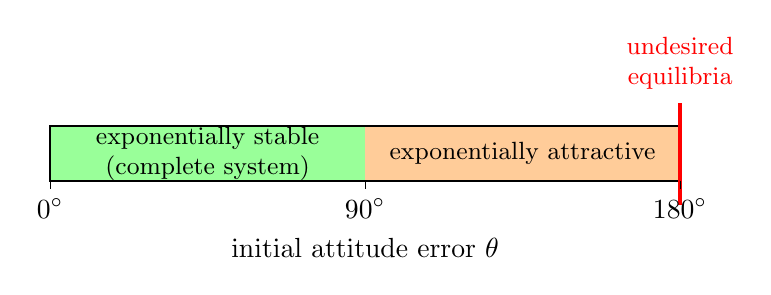
\begin{tikzpicture}[>=Stealth]
\fill[green!40] (0,0) rectangle (4,0.7);
\fill[orange!40] (4,0) rectangle (8,0.7);
\draw[thick] (0,0) rectangle (8,0.7);
\draw[red,very thick] (8,-0.3)--(8,1);
\node[font=\small,align=center] at (2,0.35) {exponentially stable\\(complete system)};
\node[font=\small,align=center] at (6,0.35) {exponentially attractive};
\node[red,font=\small,align=center] at (8,1.5) {undesired\\equilibria};
\foreach \x/\l in {0/0,4/90,8/180}{\draw (\x,0)--(\x,-0.1) node[below]{$\l^\circ$};}
\node[below] at (4,-0.6) {initial attitude error $\theta$};
\end{tikzpicture}
\caption{What the geometric controller guarantees as a function of the initial attitude error. Original figure summarizing slides~24 and 37.}
\end{figure}

\subsection{Key take-aways}

\begin{itemize}
  \item Euler angles are minimal but singular, quaternions are global but double-cover $SO(3)$ (unwinding), rotation matrices are global and unique.
  \item The quadrotor model is globally defined on $SE(3)$: design the controller there, with no local coordinates.
  \item Attitude error function $\Psi=\tfrac12\tr(I-R_d^TR)=1-\cos\theta$, errors $\eR,\eO$; closed loop $J\dot\eO=-k_R\eR-k_\Omega\eO$.
  \item Thrust = projection of the desired force on the current thrust axis: positive when the attitude error is below $90^\circ$.
  \item Stability is proved for the complete system: exponential for errors below $90^\circ$, almost global exponential attractiveness. No continuous feedback can do better on $SO(3)$ (topological obstruction).
\end{itemize}

\subsection*{References (from the slides)}
\begin{enumerate}[label={[\arabic*]},nosep]
  \item T.~Lee, M.~Leok, N.H.~McClamroch, ``Geometric tracking control of a quadrotor UAV on SE(3),'' 49th IEEE CDC, pp.~5420--5425, 2010.
  \item T.~Lee, M.~Leok, N.H.~McClamroch, ``Control of complex maneuvers for a quadrotor UAV using geometric methods on SE(3),'' arXiv:1003.2005.
  \item S.P.~Bhat, D.S.~Bernstein, ``A topological obstruction to continuous global stabilization of rotational motion and the unwinding phenomenon,'' Systems \& Control Letters 39(1), 2000.
  \item C.G.~Mayhew, R.G.~Sanfelice, A.R.~Teel, ``Quaternion-based hybrid control for robust global attitude tracking,'' IEEE TAC 56(11), 2011.
  \item J.~Stuelpnagel, ``On the parametrization of the three-dimensional rotation group,'' SIAM Review 6(4), 1964.
  \item N.A.~Chaturvedi, A.K.~Sanyal, N.H.~McClamroch, ``Rigid-body attitude control,'' IEEE Control Systems Magazine 31(3), 2011.
  \item D.~Mellinger, V.~Kumar, ``Minimum snap trajectory generation and control for quadrotors,'' IEEE ICRA, 2011.
  \item F.~Goodarzi, D.~Lee, T.~Lee, ``Geometric nonlinear PID control of a quadrotor UAV on SE(3),'' ECC 2013.
  \item B.~Siciliano et al., \emph{Robotics: Modelling, Planning and Control}, Springer, 2009 (Ch.~2).
\end{enumerate}

\end{document}
